%!TEX program = xelatex
% 完整编译方法 1 pdflatex -> bibtex -> pdflatex -> pdflatex
% 完整编译方法 2: xelatex -> bibtex -> xelatex -> xelatex
\documentclass[lang=cn,11pt]{elegantpaper}

\title{A Bipartite Network Based Recommendation System via Network Embedding Augmented Collaborative Filtering Model }

\author{袁梦祥}
\institute{安徽大学大数据与云服务工程实验室}

% 不需要版本信息,直接注释即可
% \version{0.07}
% 不需要时间信息的话,需要把 \today 删除。
\date{}


% 参考文献样式 如果想修改参考文献样式,请把这行注释掉
%\usepackage[authoryear]{gbt7714}  % 国标

% 算法表格
\usepackage{algorithm}  
\usepackage{algpseudocode}  
\usepackage{amsmath}  
\renewcommand{\algorithmicrequire}{\textbf{Input:}}  
\renewcommand{\algorithmicensure}{\textbf{Output:}}

\begin{document}

\maketitle

\begin{abstract}
\noindent 使用推荐系统为用户提供个性化的推荐服务,有助于提高用户的满意度,更好的发掘物品的“长尾”。推荐算法是推荐系统的核心,基于协同过滤的推荐算法是目前应用比较广泛的推荐算法,但传统的协同过滤算法在推荐时存在数据稀疏量大,数据维数高,无法利用内容信息等问题。为了解决协同过滤算法的缺点,本文引入了网络表示学习的方法,使用二部图网络来表示用户的行为数据和项目的内容数据,再通过学习网络中节点的低维度潜在表示,获得用户和项目的领域信息。为了结合用户和项目的领域信息对用户进行推荐,我们进一步提出了一种融合领域信息的矩阵分解技术。本文结合协同过滤和嵌入算法的优点,提出了一种新的二部图推荐系统,该系统充分考虑了不同项目的内容特征和用户的行为偏好,使用改进的矩阵分解算法对用户进行推荐。我们在GoodBooks和Movielens数据集上对此方法进行了实验验证,结果表明,与其他推荐算法相比,基于网络表示学习的加强协同过滤算法有更好的推荐效果。
\keywords{推荐系统,二部图网络,网络表示学习,矩阵分解,协同过滤 }
\end{abstract}

% \lstinline{a4paper, 10pt} 自定义命令代表强调显示
% \begin{lstlisting}  \end{lstlisting} 自定义环境 代表一个代码块

\section{介绍}

在当今竞争激烈的市场环境下,产品的个性化程度已经成为影响顾客产品选择和满意度的重要因素。如果要给用户提供个性化的商品或服务,就必须充分研究用户的兴趣,而这正是个性化推荐系统主要解决的问题。推荐系统通过挖掘用户的历史行为数据,发现用户的个性化需求,帮助企业和公司在合适的时间向合适的客户提供合适的产品和服务。

推荐系统的本质是通过一定的方式将用户和项目联系起来,因此研究怎么将用户和用户可能感兴趣的项目关联起来的推荐算法是整个推荐系统的核心。协同过滤算法是个性化推荐系统中的常用算法,计算项目的相似性是现代推荐系中的关键组成部分,与现有的工作不同,本文提出一种新的, 该系统不仅考虑

计算项目的相似性是现代推荐系统中的关键组成部分。虽然许多推荐算法专注于同时学习用户和项目的低维嵌入[1] - [2] [3],但计算项目的相似性本身就是目的。在线零售商广泛使用项目相似性来处理许多不同的推荐任务。本文通过在低维空间中嵌入项目来处理忽略学习项目相似性的任务。


与现有工作不同,本文提出了一种新的QoS感知Web服务推荐系统,该系统不仅考虑QoS度量,还考虑Web服务的功能类别。所提出的系统还可以通过采用矩阵分解方法来减少冷启动问题的影响[11],[12],该方法集成了Web服务的功能类别,并且可以比以前的方法产生更好的预测[13],[14 ] ]。

总之,本文的主要贡献有三方面:
\begin{itemize}
	\item 本论文采取表示学习的方式,学习到用户和行为的低维度向量表示,再结合矩阵分解和协同过滤的方法,实现评分预测和用户个性化推荐。
	
	\item 使用二部图表示用户的行为数据和物品的内容信息。然后,通过网络表示学习的算法,将用户根据行为数据,物品根据内容信息分别映射到不同的嵌入向量空间。最后在嵌入向量空间中比较用户之间和物品之间的相似度,利用协同过滤的思想对原始评分矩阵进行填充。
	\item 介绍由真实字Web服务QoS数据集进行的大量实验的结果,该数据集由来自20多个国家的339个用户组成,包含超过150万个Web服务调用记录。
\end{itemize}

本文的其余部分安排如下。第二节介绍了拟议的Web服务推荐系统的机制; 第三节讨论了实验研究; 第四节审查相关工作; 最后,第五节总结了论文并讨论了未来的工作。


\section{相关工作}
协同过滤推荐算法[1] 是推荐系统中最基础的算
法, 学术界有许多关于该算法的研究。该算法主要是
利用收集到的用户信息来计算它们之间的相似度, 筛
选出目标用户的邻居用户对物品的评价, 以此来预测
目标用户对物品的喜好程度。该算法不受数据格式的
影响, 可以处理复杂数据进行有效快速的推荐, 同时也
存在数据稀疏、冷启动之类的问题。
基于内容的推荐算法[3] 也是常用的算法, 该算法通
过整理用户过去喜欢的物品信息, 找出与之相似度高的
物品对目标用户进行推荐。该算法在计算物品相似度的基础上分析用户和物品的内部信息, 通过用户的喜好
和物品的属性来进行推荐。该算法在考虑用户喜好的
同时也达到了推荐结果直观且便于理解的作用。但是
该算法处理非文本信息难度比较高, 比如音乐、图像等。
组合推荐算法[5 - 6] 是通过结合多种推荐算法来实
现推荐。协同过滤推荐和基于内容的推荐都有一定的局
限性, 在实际应用中, 通常将多种推荐算法结合起来使用,
这样可以达到更好的效果。例如将以上两种算法组合使
用就可以取长补短, 组合推荐算法往往比单一的推荐算
法有更高的准确率, 但是时间以及空间开销也因此增加。
基于网络结构的推荐算法[7 - 8] 不考虑用户和物品
的信息, 而是将用户与物品抽象为网络中的节点, 用户
与物品的关系隐藏在网络的连接中, 该算法利用网络
结构构成的信息进行推荐。Zhou 等[9] 提出基于二部
图网络的推荐算法, 该方法在复杂网络物质扩散和热
传导思想上得到启发, 用资源分配的方法来计算用户
间的相似性, 取得了比其他算法更好的效果。在此基
础上, 将用户对项目的评分作为边权, 提出了基于加权
的二部图推荐算法[10 - 11] , 算法得到了进一步的优化。
本文考虑到各个算法的优缺点, 将基于物品的协
同过滤算法与结合初始资源配置的加权二部图网络推
荐算法融合到一起, 提高了推荐的效果。

二部网络是一种普遍存在的数据结构,用于对两类实体之间的关系进行建模。它在推荐系统、搜索引擎、问答系统等方面得到了广泛的应用。例如,在搜索引擎中,查询和网页形成一个二部图网络,边缘可以指示用户点击行为,提供有价值的关联信号[1,2];在推荐系统的另一个应用中,用户和项目形成一个二部网络,边缘可以编码包含丰富的协同过滤模式[3]的用户评价行为。要对网络数据执行预测分析,首先获得表示形式(即,特征向量)表示顶点。传统的向量空间方法,如袋装词表示方法,在处理大规模动态网络的实际应用中,语义捕获太少,效率低下。近年来,数据挖掘和信息检索领域的研究主要集中在从数据中学习表示[4 7]。特别是,它们将顶点嵌入到低维空间中,即,将顶点表示为可学习的嵌入向量。基于顶点嵌入的标准机器学习技术可以应用于各种预测任务,如顶点标记、链接预测、聚类等。

\begin{enumerate}
	\item \lstinline{协同过滤}:介绍传统的协同过滤算法
	\item \lstinline{LFM 矩阵分解}:使用机器学习的方式解决推荐问题
	\item \lstinline{item2Vec}:更进一步 使用深度学习的方式解决推荐问题
\end{enumerate}


\section{推荐模型}
使用图嵌入的方式,将用户-物品的二部图表示转化为低维度的向量,在低维度向量空间中,考虑相似性,最后结合矩阵分解和协同过滤模型,通过机器学习的方式填充评分矩阵,完成个性化推荐。

融合领域信息的矩阵分解的loss函数如下:


\subsection{算法}

这里介绍模型使用的算法

\begin{algorithm}[h]  
	\caption{Conjugate Gradient Algorithm with Dynamic Step-Size Control}  
	\label{alg::conjugateGradient}  
	\begin{algorithmic}[1]  
		\Require  
		$f(x)$: objective funtion;  
		$x_0$: initial solution;  
		$s$: step size;  
		\Ensure  
		optimal $x^{*}$  
		\State initial $g_0=0$ and $d_0=0$;  
		\Repeat  
		\State compute gradient directions $g_k=\bigtriangledown f(x_k)$;  
		\State compute Polak-Ribiere parameter $\beta_k=\frac{g_k^{T}(g_k-g_{k-1})}{\parallel g_{k-1} \parallel^{2}}$;  
		\State compute the conjugate directions $d_k=-g_k+\beta_k d_{k-1}$;  
		\State compute the step size $\alpha_k=s/\parallel d_k \parallel_{2}$;  
		\Until{($f(x_k)>f(x_{k-1})$)}  
	\end{algorithmic}  
\end{algorithm}  




\subsection{算法模型图}

介绍算法的模型

\begin{figure}[h]
	\centering
	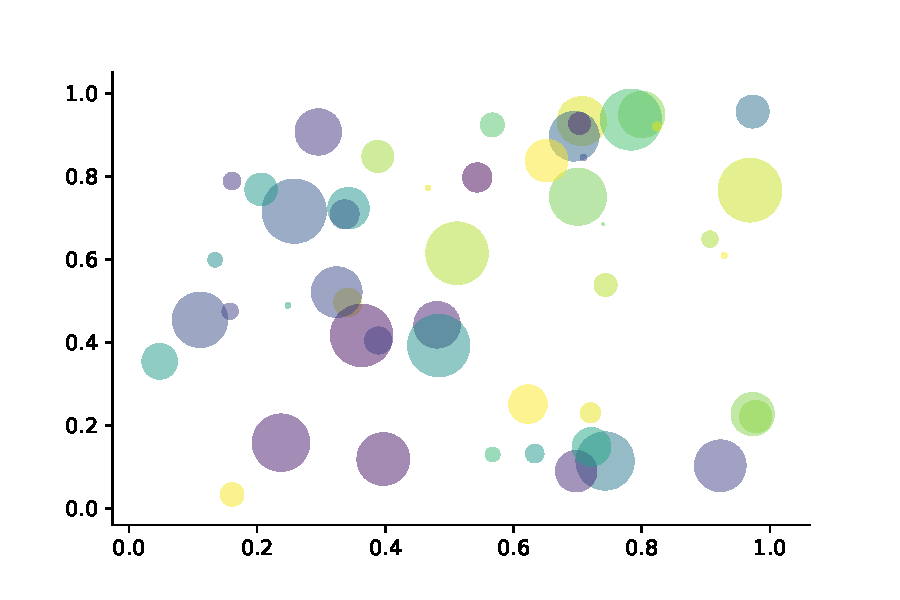
\includegraphics[width=0.6\textwidth]{imgs/scatter.pdf}
	\caption{Scatter Plot Example \label{fig:scatter}}
\end{figure}


\section{实验}
实验部分,介绍论文的实验

我强烈建议你使用 \lstinline{booktabs} 宏包,这个宏包有三个命令 \lstinline{\toprule}、\lstinline{\midrule} 和 \lstinline{\bottomrule} 能方便你制作三线表。\tabref{tab:reg} 是一个示例:

\begin{table}[h]
	\centering
	\caption{Auto MPG and Price \label{tab:reg}}
	\begin{tabular}{lcc}
		\toprule
		&       (1)         &        (2)      \\
		\midrule
		mpg             &    -238.90***     &      -49.51     \\
		&     (53.08)       &      (86.16)    \\
		weight          &                   &      1.75***    \\
		&                   &      (0.641)    \\
		constant        &     11,253***     &       1,946     \\
		&     (1,171)       &      (3,597)   \\
		obs             &        74         &         74     \\
		$R^2$           &      0.220        &       0.293    \\
		\bottomrule
		\multicolumn{3}{l}{\scriptsize Standard errors in parentheses} \\
		\multicolumn{3}{l}{\scriptsize *** p<0.01, ** p<0.05, * p<0.1} \\
	\end{tabular}%
\end{table}%

\section{结论和未来工作}
结论部分,介绍论文的实验结果

%\nocite{*} 代表显示所有的论文文献 包括文中没有引用的

% 如果想修改参考文献样式(非国标),请把下行取消注释,并换成合适的样式(比如 unsrt,plain 样式)。
\bibliographystyle{unsrt}
\bibliography{wpref}

\end{document}
